\documentclass{beamer}
\mode<presentation>
\setbeamertemplate{navigation symbols}{}

\usepackage{tikz}
\usetikzlibrary{spy}
\usepackage{algpseudocode}
%\includeonlyframes{small}
%\algrenewcommand\algorithmicindent{0.5em}
\algtext*{EndFor}% Remove "end while" text
\algtext*{EndIf}% Remove "end if" text
\algtext*{EndProcedure}% Remove "end procedure" text

% Needed for diagrams.
\def\im#1#2{
  \node(#1) [scale=#2]{\pgfbox[center,top]{\pgfuseimage{#1}}
};}
\newcommand{\air}{\vspace{0.5cm}}
\pgfdeclareimage{dot}{diagrams/dot}
\pgfdeclareimage{dots1}{animations/dots1}
\pgfdeclareimage{dots2}{animations/dots2}
\pgfdeclareimage{dots3}{animations/dots3}
\pgfdeclareimage{DP_Output}{diagrams/DP_Output}
\pgfdeclareimage{DP_class}{diagrams/DP_class}
\pgfdeclareimage{dep_score}{diagrams/dep_score}
\pgfdeclareimage{dependency_rules}{diagrams/dependency_rules}
\pgfdeclareimage{dp_mistake}{diagrams/dp_mistake}
\pgfdeclareimage{dyna_dep}{diagrams/dyna_dep}
\pgfdeclareimage{eisner_paper}{diagrams/eisner_paper}
\pgfdeclareimage{implementation}{diagrams/implementation}
\pgfdeclareimage{parse_hypergraph}{diagrams/parse_hypergraph}
\pgfdeclareimage{parse_hypergraph_no_path}{diagrams/parse_hypergraph_no_path}
\pgfdeclareimage{parse_hypergraph_no_path_1}{diagrams/parse_hypergraph_no_path_1}
\pgfdeclareimage{ryan_imperative}{diagrams/ryan_imperative}
\pgfdeclareimage{single_edge}{diagrams/single_edge}
\pgfdeclareimage{dot}{diagrams/dot}
\pgfdeclareimage{edge}{diagrams/edge}
\pgfdeclareimage{full}{diagrams/full}
\pgfdeclareimage{full_trans}{diagrams/full_trans}
\pgfdeclareimage{full_trans_color}{diagrams/full_trans_color}
\pgfdeclareimage{parse_firstorder1}{diagrams/parse_firstorder1}
\pgfdeclareimage{parse_firstorder2}{diagrams/parse_firstorder2}
\pgfdeclareimage{parse_firstorder3}{diagrams/parse_firstorder3}
\pgfdeclareimage{parse_firstorder4}{diagrams/parse_firstorder4}
\pgfdeclareimage{parse_firstorder5}{diagrams/parse_firstorder5}
\pgfdeclareimage{parse_firstorder6}{diagrams/parse_firstorder6}
\pgfdeclareimage{parse_firstorder7}{diagrams/parse_firstorder7}
\pgfdeclareimage{parse_firstorder8}{diagrams/parse_firstorder8}
\pgfdeclareimage{parse_firstorder9}{diagrams/parse_firstorder9}
\pgfdeclareimage{parse_firstorder_heat1}{diagrams/parse_firstorder_heat1}
\pgfdeclareimage{parse_firstorder_heat2}{diagrams/parse_firstorder_heat2}
\pgfdeclareimage{parse_firstorder_heat3}{diagrams/parse_firstorder_heat3}
\pgfdeclareimage{parse_firstorder_heat4}{diagrams/parse_firstorder_heat4}
\pgfdeclareimage{parse_firstorder_heat5}{diagrams/parse_firstorder_heat5}
\pgfdeclareimage{parse_firstorder_heat6}{diagrams/parse_firstorder_heat6}
\pgfdeclareimage{parse_firstorder_heat7}{diagrams/parse_firstorder_heat7}
\pgfdeclareimage{parse_firstorder_heat8}{diagrams/parse_firstorder_heat8}
\pgfdeclareimage{parse_firstorder_heat9}{diagrams/parse_firstorder_heat9}


\title{Dynamic Programming: Theory and Practice}
\author{Alexander Rush and Nathaniel Filardo\\ MASC 2013}

\begin{document}

\begin{frame}
  \titlepage
\end{frame}

\begin{frame}
  So I've been working with a student. 

  \pause
  \air

  And I ask her to build a dependency parser.

\air 
\pause  

  ``What should I use to write that?''
\end{frame}

\bgroup
\setbeamercolor{background canvas}{bg=black}

\begin{frame}[t]
  \begin{figure}
    \centering
    \begin{tikzpicture}
      \im{DP_class}{0.35}
    \end{tikzpicture}
  \end{figure}
  
  \vspace{6cm}

  \begin{center}
    \textcolor{white}{when I am in my advisor's class}    
  \end{center}

\end{frame}

\begin{frame}[t]
  \begin{figure}
    \centering
    \begin{tikzpicture}
      \im{eisner_paper}{0.4}
    \end{tikzpicture}    
  \end{figure}

  \vspace{6cm}

  \begin{center}
    \textcolor{white}{when I read the paper}
  \end{center}

\end{frame}

\begin{frame}[t]
  \vspace{-1cm}
  \begin{figure}
    \centering
    
\begin{tikzpicture}
      \im{implementation}{0.25}
    \end{tikzpicture}
  \end{figure}

  \vspace{7.5cm}

  \begin{center}
    \textcolor{white}{when I look at the code}
  \end{center}
\end{frame}

\bgroup
\setbeamercolor{background canvas}{bg=white}

% \begin{frame}{Story}
% \end{frame}


\begin{frame}{Question}
  We no longer manually implement 
  \begin{itemize}    
    \air 
  
    \item Simplex for LPs
      \air

    \item SVM training for classification
      \air
      
    \item FST algorithms
      \air 

    \item etc. 
  \end{itemize}
  \pause 
  \air
  But I don't have a good answer for dynamic programming.
\end{frame}

\begin{frame}
  \frametitle{Outline}
  Four views of Dynamic Programming
  \begin{enumerate}
  \item Imperative
    \air
k
  \item Declarative
    \air
  \item Graphical
    \air 
  \item Optimization
  \end{enumerate}
\end{frame}

\begin{frame}
  \begin{center}
    \Large{Dynamic Programming for NLP}
  \end{center}
\end{frame}

\begin{frame}[c]
  \frametitle{Decoding for NLP}

  \begin{itemize}
  \item $f$; a scoring function.
  \item $y$; a possible output structure.  
  \end{itemize}

  \textbf{optimization problem:} 
  \[ \max_{y} f(y) \]

\end{frame}

\begin{frame}[t]{Example: Dependency Parsing}   
   \begin{figure}
     \centering
     \begin{tikzpicture}
       \im{dep_score}{0.35}
     \end{tikzpicture}
   \end{figure}
\end{frame}

\begin{frame}
  \frametitle{Dynamic Programming for Decoding}

  ``Dynamic programming is a method for solving complex problems by breaking them down into simpler subproblem''
  
  \air 
  Traditionally defined as an optimization problem defined using the Bellman equations.

  \air
  However these equations don't give use much insight into what to do in practice.

\end{frame}


\begin{frame}
  \begin{center}
    \Large{View 1: Imperative}
  \end{center}
\end{frame}

\begin{frame}
  In my advisor's class, we teach an imperative implementation of dynamic programming using charts. 

\air 

\pause 

Some students enjoy this, it correlates well with not having bugs.
\end{frame}

\bgroup
\setbeamercolor{background canvas}{bg=black}

\begin{frame}[t]
  \begin{figure}
    \centering
    \begin{tikzpicture}
      \im{ryan_imperative}{0.65}
    \end{tikzpicture}
  \end{figure}
\end{frame}

\bgroup
\setbeamercolor{background canvas}{bg=white}

\begin{frame}
  \frametitle{Benefits}
  \begin{itemize}
  \item Often fastest method in practice.  
    \air 

  \item Doesn't require any additional code or library.
    \air

  \item Great way to prove how hardcore you are.
  \end{itemize}
\end{frame}

% \begin{frame}{Sample Animation} 
%   \begin{tikzpicture}
%      \foreach \x in {1,...,3} {
%        \uncover<\x>{\im{dots\x}{1.0}}
%      }        
%   \end{tikzpicture}
% \end{frame}

\begin{frame}[t]{Issue 1}
  \begin{itemize}
  \item Debugging is very subtle.
  \end{itemize}


  \begin{figure}
    \centering
    \begin{tikzpicture}
      \im{dp_mistake}{0.7}
    \end{tikzpicture}
  \end{figure}


\end{frame}

\bgroup
\setbeamercolor{background canvas}{bg=black}

\begin{frame}[t]
  \vspace{-1.2cm}
  \begin{figure}
    \centering
    \begin{tikzpicture}
      \im{DP_Output}{0.4}
    \end{tikzpicture}
  \end{figure}
\end{frame}

\bgroup
\setbeamercolor{background canvas}{bg=white}

\begin{frame}{Issue 2}
  \begin{itemize}
  \item Optimized to the specific problem domain.
  \end{itemize}
  \air 

  Cannot use MSTParser for POS tagging. 
  \pause 
  \air

  Cannot really use MSTParser third-order parsing. 

\end{frame}



\begin{frame}{Issue 3}
  Cannot easily utilize dynamic programming extensions.

  \begin{itemize}
    \item Variant algorithms
      \begin{itemize}
        \item K-Best
        \item Loss-Augmented inference
        \item Posterior Decoding
      \end{itemize}
      \pause 
      \air 

    \item Pruning algorithms
      \begin{itemize}
      \item Max-Marginals
      \item Coarse-to-Fine
      \end{itemize}

      \pause 
      \air 

    \item Constrained algorithms
      \begin{itemize}
      \item Beam Search
      \item Dual Decomposition
      \item Lagrangian Relaxation
      \end{itemize}
      ....
  \end{itemize}
\end{frame}

\begin{frame}
  \frametitle{Opinion Slide}
  Do not write imperative dynamic programming code.
\end{frame}

\begin{frame}
  \begin{center}
    \Large{View 2: Declarative}
  \end{center}
\end{frame}

\begin{frame}{Dependency Parsing Setup}
  \vspace{-4cm}
  \begin{figure}
    \centering
    \begin{tikzpicture}
      \im{dependency_rules}{0.35}
    \end{tikzpicture}
  \end{figure}
\end{frame}


\begin{frame}[c]{First-Order Parsing}
  \vspace{-3cm}
  \begin{figure}
    \centering
    \begin{tikzpicture}
      \foreach \x in {1,...,9} {
        %\begin{scope}[yshift=1cm]
          \uncover<\x>{\im{parse_firstorder\x}{1.0}}
        %\end{scope}
      }
    \end{tikzpicture} 
  \end{figure}
\end{frame}



\begin{frame}[fragile]
  Declarative code is clean, often less buggy.
  \air 

  \begin{small}
  \begin{verbatim}
:- item(item, double, 0).
:- item([lhalf,rhalf,end], bool, false).
constit(A,H,H,H) += rewrite(A:D,D) if word(D,H).
left(A/C,I,J,H) += constit(B,I,H2,J) * rewrite(A:D,B:D2,C:D) 
if lhalf(C,=J+1,H) & word(D,H) & word(D2,H2).
right(A\C,H,I,J) += constit(B,I,H2,J) * rewrite(A:D,C:D,B:D2) 
if rhalf(C,H,=J-1) & word(D,H) & word(D2,H2).
lhalf(A,I,H) |= constit(A,I,H,J)!=0.
rhalf(A,H,J) |= constit(A,I,H,J)!=0.
constit(A,I,H,K) += left(A/C,I,J,H) * constit(C,=J+1,H,K). 
constit(A,I,H,K) += constit(C,I,H,=J-1) * right(A\C,H,J,K).
goal += constit(s,1,_,N) if end(N).
  \end{verbatim}
  \end{small}
  % \begin{figure}
  %   \centering
  %   \begin{tikzpicture}
  %     \im{dyna_dep}{0.3}
  %   \end{tikzpicture}
  % \end{figure}

  \pause

  I am not smart enough to make this efficient. 

\end{frame}

% \bgroup
% \setbeamercolor{background canvas}{bg=black}

% \begin{frame}[c]
%   \vspace{-1cm}
%   \begin{figure}
%     \centering
%     \begin{tikzpicture}
%       \im{dyna_dep}{0.3}
%     \end{tikzpicture}
%   \end{figure}
% \end{frame}

% \bgroup
% \setbeamercolor{background canvas}{bg=white}

\begin{frame}
  \begin{center}
    \Large{View 3: Hypergraph}
  \end{center}
\end{frame}

\begin{frame}[t]{Hyperedge}
  \begin{figure}
    \centering
    \begin{tikzpicture}
      \im{single_edge}{0.5}
    \end{tikzpicture}
  \end{figure}
\end{frame}

\begin{frame}{Hypergraph}
  \begin{table}
    \centering
    
  \begin{tabular}{llll}
    ${\cal V}$ & set of vertices &    1 & root node \\
    ${\cal E}$ & set of hyperedges &   $h(e)$ &  head vertex of edge \\
   && $t(e)$ & tail vertex of edge \\
   \end{tabular}
  \end{table}

  \begin{itemize}
  \item ${\cal X}$ - set of valid ``hyperpaths'' $y$ 
    \begin{itemize}
    \item $y \in \{ 0,1 \}^{|{\cal V}| + |{\cal E}|}$ has $y(v) = 1$ iff node $v$ is in path
    \end{itemize}
  \end{itemize}

  \air 
  Any dynamic program can be represented as a hypergraph. 
\end{frame}

\begin{frame}[t]
  \vspace{-1cm}
  \begin{figure}
    \centering
    \begin{tikzpicture}
      \im{parse_hypergraph_no_path}{0.17}
    \end{tikzpicture}
  \end{figure}
\end{frame}


% \begin{frame}[t,label=small]
%   \frametitle{}
%   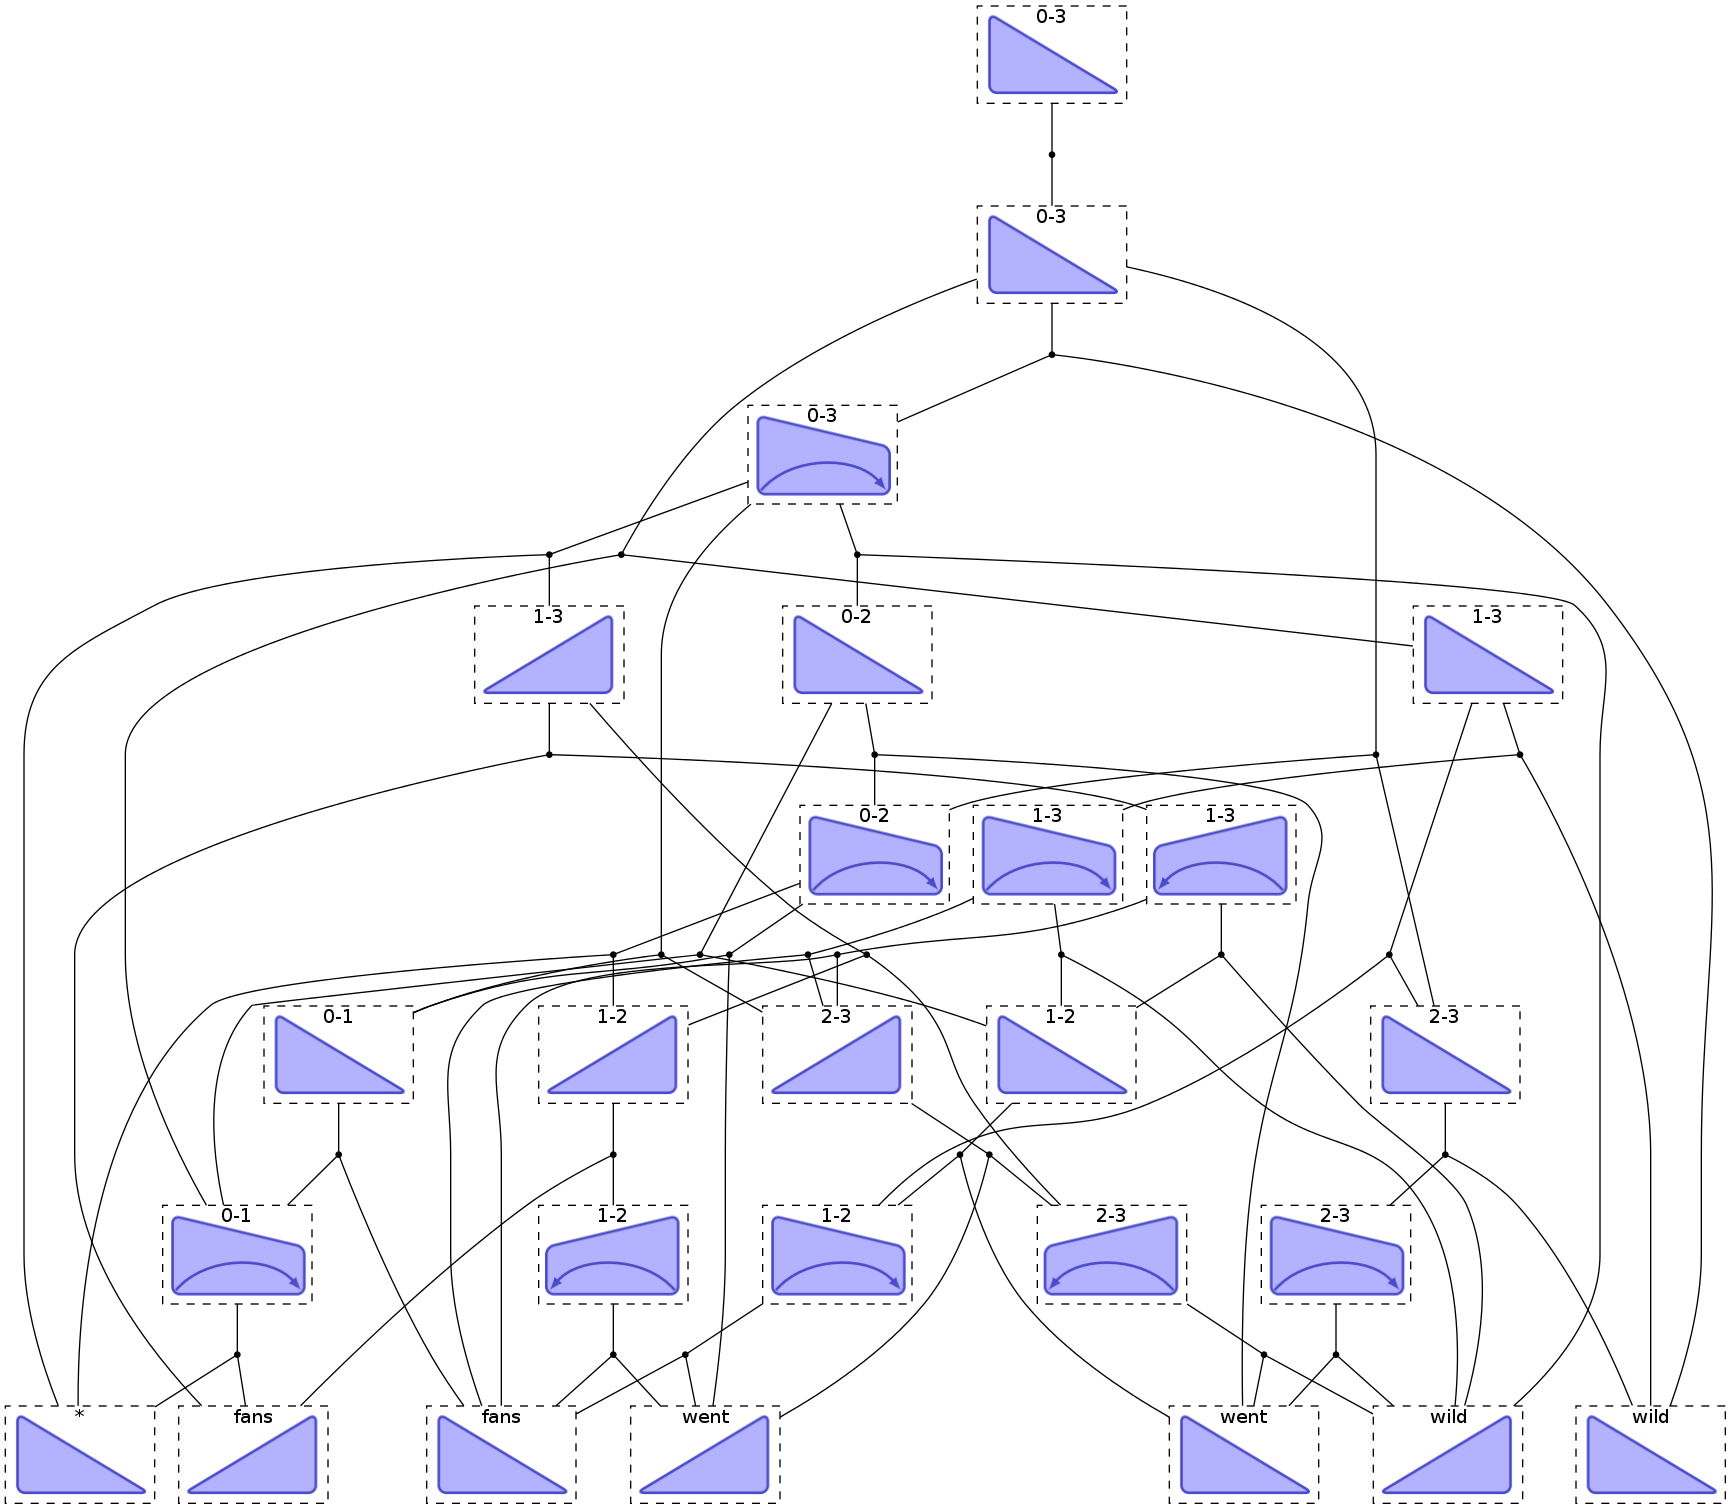
\includegraphics[height=\textheight,width=\textwidth, keepaspectratio]{diagrams/parse_hypergraph_no_path}
%   \framezoom<2><3>[border=4](2.5cm,7cm)(2.5cm,2.5cm)

%   \framezoom<4><5>[border=4](5.3cm,5cm)(2.5cm,2.5cm)
% \end{frame}


\begin{frame}[label=small]
  \begin{tikzpicture}[
    spy using outlines={
      circle,
      magnification=2,
      size=6cm,
      connect spies}]

    \node[inner sep=0pt] {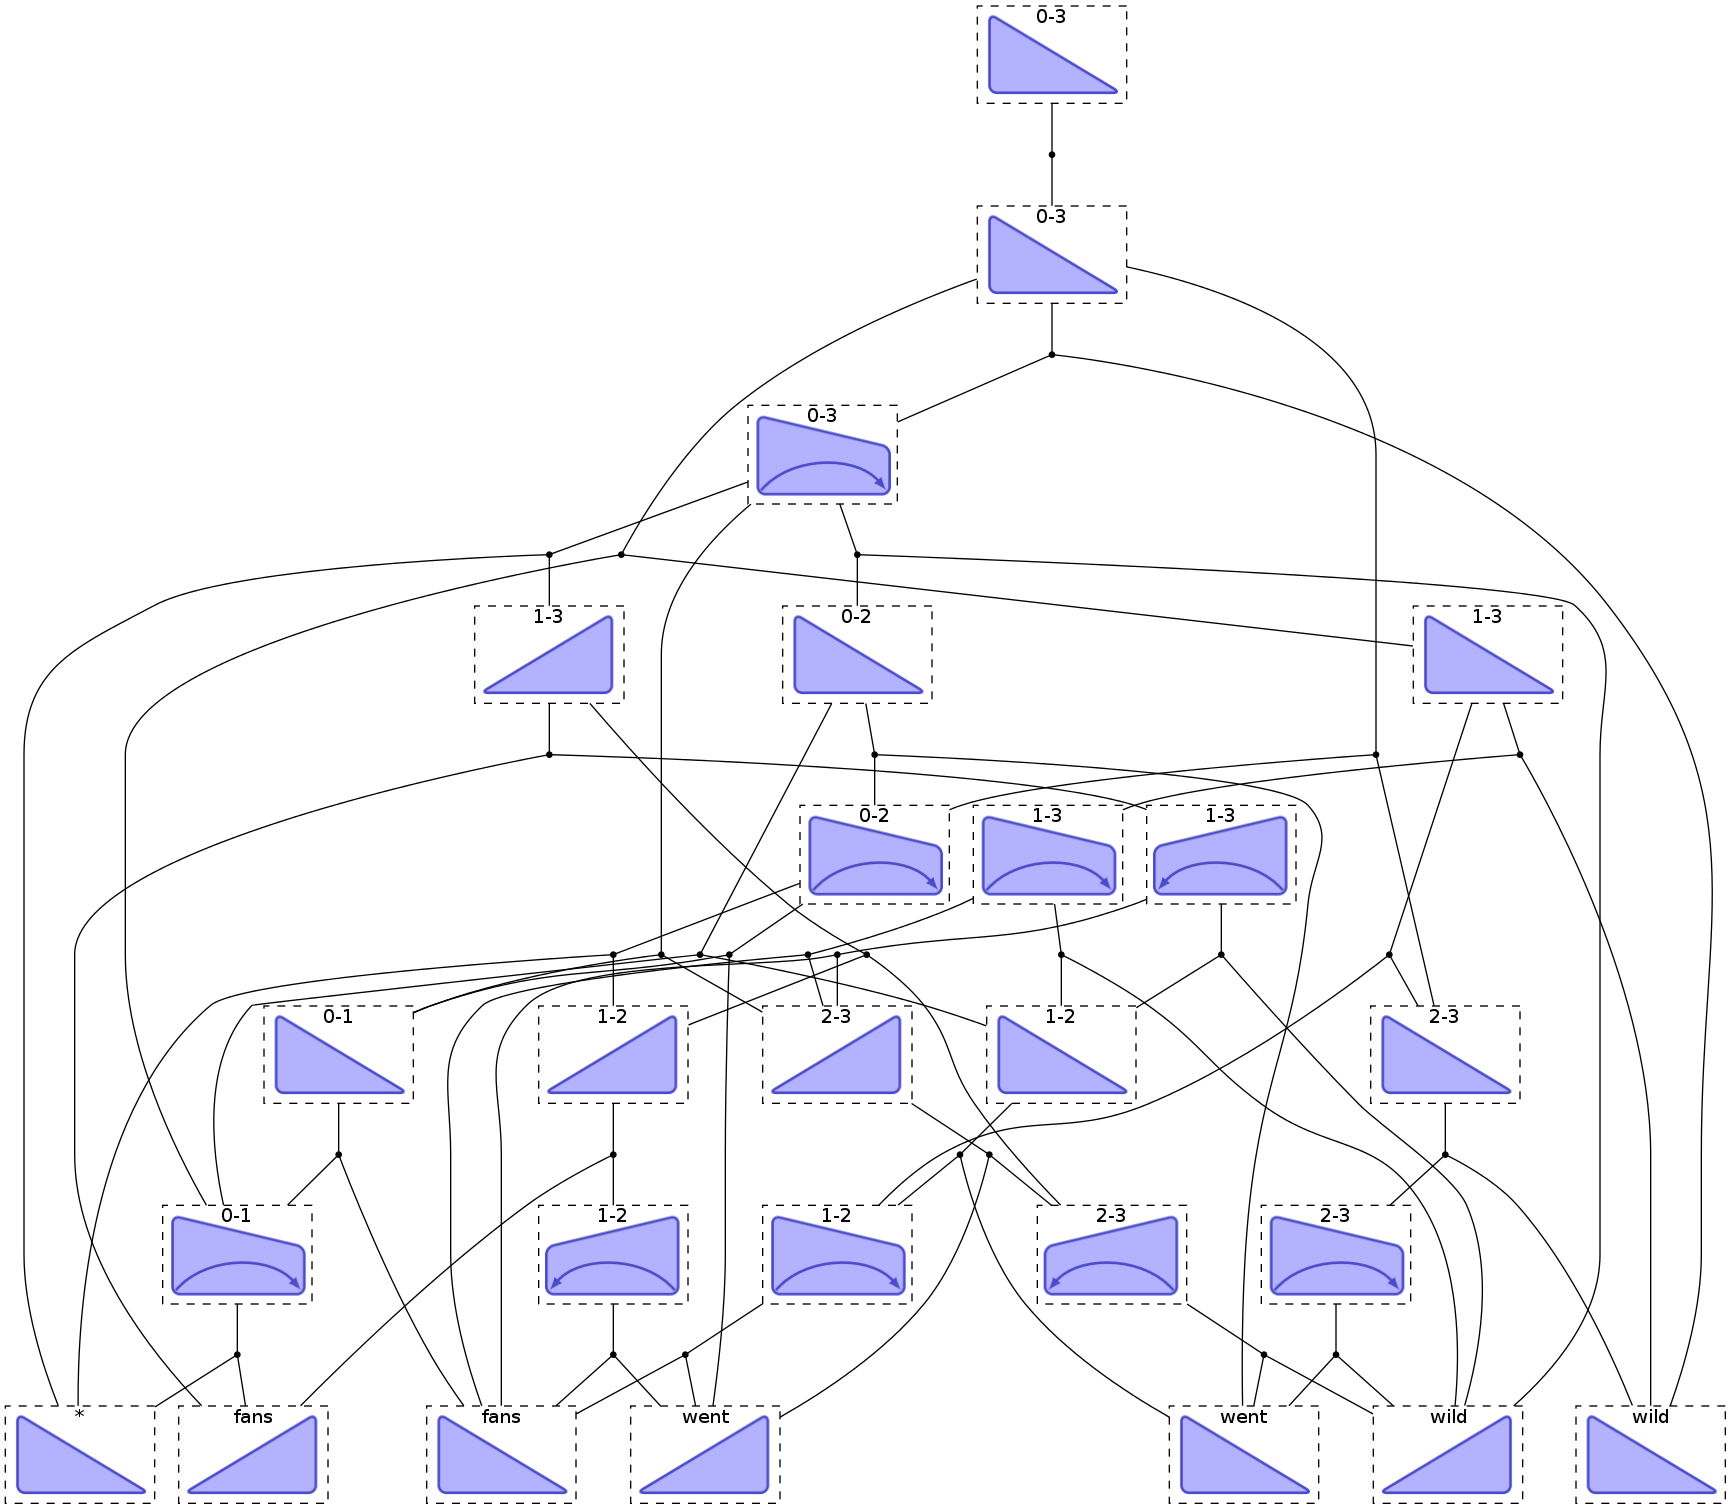
\includegraphics[width=\textwidth]{diagrams/parse_hypergraph_no_path}};
    \only<2>{\spy[red!70!black] on (-1.5,-4) in node at (-3, 2);}
    \only<3>{\spy[red!70!black] on (1.5,-1) in node at (-3, 2);}
  \end{tikzpicture}
\end{frame}

\begin{frame}{Weights}
  \begin{itemize}
  \item $\theta \in R^{|{\cal E}|}$ - the weights associated with each hyperedge. 
  \end{itemize}

  \air 

  \textbf{Hypergraph problem}: 
  \[ \max_{y \in {\cal X}} \theta^\top y \]
\end{frame}

\begin{frame}{Dynamic Programming on Hypergraphs}
  \begin{algorithmic}
    \Procedure{BestPath}{${\cal V}, {\cal E}, {\theta}$}
    \State{$\pi(v) \gets 0$ for all terminals}
    \For{$v \in {\cal V}$ in bottom-up order}
    \State{$\displaystyle \pi(v) \gets \max_{e \in {\cal E} : h(e) = v} \theta(e) +  \pi(t(e))$}
    \EndFor{}
    \Return{$\pi(1)$}
    \EndProcedure{}
  \end{algorithmic}
\end{frame}


\begin{frame}[t]
  \vspace{-1cm}
  \begin{figure}
    \centering
    \begin{tikzpicture}
      \im{parse_hypergraph}{0.17}
    \end{tikzpicture}
  \end{figure}
\end{frame}

\begin{frame}
\begin{algorithmic}
\Procedure{Outside}{${\cal V}, {\cal E}, {\theta}$}
\State{$\rho[1] \gets 0$}
\For{$e \in {\cal E}$ in top-down order}
\State{$\langle \langle v_2, \ldots, v_k \rangle,  v_1 \rangle \gets e$}
\State{$\displaystyle 
  t \gets \theta(e) + \sum_{i = 2}^k \pi[v_i]$}
\For{$i = 2 \ldots k$}
\State{$s \gets \rho[v_1] + t - \pi[v_i]$}
\If{$s > \rho[v_i]$} $\rho[v_i] \gets s$
\EndIf{}
\EndFor{}
\State{\Return{$\rho$}}
\EndProcedure{}
\end{algorithmic}
\end{frame}

\begin{frame}{Benefits}
  \begin{itemize}
  \item Helps debugging, visualizing, pruning, and explaining.
    \air 
  \item Can optimize the hell out of the inner loop code.
    \air 
  \item Useful for other downstream tasks.
  \end{itemize}
\end{frame}

\begin{frame}{Caveats}
  \begin{itemize}
  \item Need to create edges in memory.
    \air 
  \item Requires construction, often still imperative. 
  \end{itemize}
\end{frame}

\begin{frame}
  \begin{center}
    \Large{View 4: Optimization}
  \end{center}
\end{frame}

\begin{frame}{Linear Program}
  \begin{itemize}
    \item
      Any dynamic program can be expressed as a linear program. 
      \air 

    \item
      Can be derived from the Bellman equations.
  
      \air 
    \item Also directly from the hypergraph representation.

   \end{itemize}
\end{frame}

\begin{frame}{Linear Constraints Conversion}
  \begin{eqnarray*}
  {\cal X} = \{ y : y(1) &=& 1, \\
  y(v) &=& \sum_{e : h(e) = v} y(e)\ \forall \ v \in {\cal V} \mbox{ except root},  \\
  y(v) &=& \sum_{e : t(e)= v} y(e)\ \forall \ v \in {\cal V} \mbox{ except terminals} \} \\
\end{eqnarray*}
\pause
\begin{itemize}
  \item$O(|{\cal V}|)$ constraints
\end{itemize}
\end{frame}

\begin{frame}{Linear Program}
  \[ \max_{y} \theta^\top y\] 

  \begin{eqnarray*}
  y(1) &=& 1 \\
  y(v) &=& \sum_{e : h(e) = v} y(e)\ \forall \ v \in {\cal V} \mbox{ except root}  \\
  y(v) &=& \sum_{e : t(e)= v} y(e)\ \forall \ v \in {\cal V} \mbox{ except terminals}  \\
  0 \leq &y(e) & \leq 1\ \  \forall e \in {\cal E} \\
  0 \leq &y(v) &\leq 1 \ \  \forall v \in {\cal V} \\
\end{eqnarray*}
\end{frame}

\begin{frame}[fragile]
  \begin{small}
\begin{verbatim}
\* Hypergraph Problem *\
Minimize
OBJ: 0.865309927772 edge_0 + 0.805027827013 edge_1 + 0.719704686404 edge_2
 + 0.824844977148 edge_3 + 0.668153201232 edge_4 + 0.932833824227 edge_5
 + 0.551267246091 edge_6
Subject To
_C1: node_13_tri_right_0_3 = 1
_C10: - edge_0 + node_1_tri_right_1_1 = 0
_C11: - edge_1 + node_2_tri_left_1_1 = 0
_C12: - edge_2 + node_3_tri_right_2_2 = 0
_C13: - edge_0 + node_4_tri_left_2_2 = 0
_C14: - edge_3 + node_5_tri_right_3_3 = 0
_C15: - edge_2 + node_6_tri_left_3_3 = 0
_C16: - edge_1 + node_7_trap_left_1_2 = 0
_C17: - edge_4 + node_8_tri_left_1_2 = 0
_C18: - edge_3 + node_9_trap_right_2_3 = 0
\end{verbatim}
    \ldots
  \end{small}
\end{frame}


\begin{frame}{Benefits}
  \begin{itemize}
  \item Can solve with general-purpose LP solver. (Gurobi)
    \air 

  \item There are tricks for outside, K-Best, etc. 
    \air 
  \item Real benefit: Adding additional constraints.
  \end{itemize}
\end{frame}


\begin{frame}[label=current]{Constrained Paths}
  \textbf{problem:} constrain maximization to valid paths
  \begin{itemize}
  \item $A \in \Reals^{|b| \times |{\cal E}|}$; a matrix of linear constraints
  \item $b \in \Reals^{|b|}$; a constraint vector
  \end{itemize}
  
  \air 
  Constrained paths
  \[ {\cal X}' = \{y \in {\cal X} : A y = b \} \]

  Constrained best path
  \[   \max_{ y \in \alert{{\cal X}'}} \theta^{\top} y  \]
\end{frame}

\begin{frame}[t]{Individual Edge ($e$)}
  \begin{figure}
    \centering
    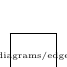
\begin{tikzpicture}
      \im{edge}{0.6}
    \end{tikzpicture}
  \end{figure}
  \vspace{3cm}

  \begin{eqnarray*}
 \theta(e) &=& \hbox{score}(\hbox{diese kritik}, \hbox{this criticism}) + \\
&&\hbox{score}(\hbox{must}, \hbox{this}) + \hbox{score}(\hbox{this}, \hbox{criticism})
  \end{eqnarray*}

\end{frame}

\begin{frame}{Constraints}
  \vspace{-3cm}
  \begin{figure}
    \centering
    \begin{tikzpicture}
      \im{full_trans}{0.37}
    \end{tikzpicture}
  \end{figure}
\end{frame}

\begin{frame}{Constraints}
  \vspace{-3cm}

  \begin{figure}
    \centering
    \begin{tikzpicture}
      \im{full_trans_color}{0.37}
    \end{tikzpicture}
  \end{figure}
\end{frame}

\begin{frame}{}
  
\end{frame}

\begin{frame}{Pitch: PyDecode}
  A pragmatic library for building dynamic programming. 

  \begin{itemize}
  \item Easy interface in Python
  \item Hypergraph code in C++
    \begin{itemize}
    \item Inside/Outside Viterbi
    \item Pruning with max-marginals
    \item Constraint specification 
    \item Dual Decomposition/Lagrangian Relaxation 
    \item Export to LP
    \end{itemize}
  \item Visualization tools supporting IPython Notebook
  \end{itemize}
\end{frame}

\end{document}

%%% Local Variables: 
%%% mode: latex
%%% TeX-master: t
%%% End: 